\documentclass[11pt,professionalfonts]{beamer}
\usefonttheme{serif}

\usepackage{presentation_packages}
\bibliography{library} % must be in the preamble when using biblatex package

\definecolor{mygray}{gray}{0.9}
\definecolor{RoyalBlue}{rgb}{0.25,0.41,0.88}
\def\Emph{\textcolor{RoyalBlue}}

\definecolor{tmp}{rgb}{0.804,0.941,1.0}
\setbeamercolor{numerical}{fg=black,bg=tmp}
\setbeamercolor{exact}{fg=black,bg=red}

\mode<presentation> 
{
  \usetheme{Warsaw}
  \usefonttheme{serif}
  \setbeamercovered{transparent}
}

\setbeamertemplate{footline}%{split theme}
{%
  \leavevmode%
  \hbox{\begin{beamercolorbox}[wd=.5\paperwidth,ht=2.5ex,dp=1.125ex,leftskip=.3cm,rightskip=.3cm plus1fill]{author in head/foot}%
    \usebeamerfont{author in head/foot}\insertshorttitle
  \end{beamercolorbox}%
  \begin{beamercolorbox}[wd=.5\paperwidth,ht=2.5ex,dp=1.125ex,leftskip=.3cm,rightskip=.3cm]{title in head/foot}
%    \usebeamerfont{title in head/foot}\mypaper\hfill \insertframenumber/\inserttotalframenumber
    \usebeamerfont{title in head/foot}\hfill \insertframenumber/\inserttotalframenumber
  \end{beamercolorbox}}%
  \vskip0pt%
} \setbeamercolor{box}{fg=black,bg=yellow}


\title[Lesson 01 - Introduction]{\large \textbf{Introduction and Overview}}

\author{\vspace*{-0.3cm}}

   
\institute{
  \footnotesize
  {\normalsize\bf{Shankar Kulumani}}\\
  \vspace*{0.2cm}
    \textbf{Flight Dynamics \& Control Lab}\\ \vspace*{0.5cm}
  \begin{figure} %figure%
        
\includegraphics[width=0.75\textwidth]{figures/gw_txh_2cs_pos.pdf}
    \end{figure}
}
\date{}

\begin{document}
%=======================================================%

\setcounter{framenumber}{-1}
\begin{frame} %-----------------------------%
  \titlepage
\end{frame}   %-----------------------------%

\section*{}
\subsection*{Introduction}  

\begin{frame}{Overview}
    \begin{itemize}
        \item Projects Overview
        \item Programming Guidelines
        \item Course Goals
            \begin{itemize}
                \item Use high-level programming language to solve engineering problems that will be encountered in engineering courses
                \item Course will focus on computer programming for astrodynamics
                \item Emphasis on well documented, structured programming, debugging and unit testing to verify that code is correct
            \end{itemize}
    \end{itemize}
\end{frame}

\begin{frame}{My Background}
    \begin{itemize}
        \item 2009 US Air Force Academy, 2013 Purdue, 2018-ish GWU
        \item Astronautical Engineer USAF 
            \begin{itemize}
                \item ORS-1 - Managed spacecraft development
                \item ANGELS - Autonomous rendezvous and orbit determination
            \end{itemize}
        \item Research in dynamics and controls
    \end{itemize}
    \begin{columns}
        \begin{column}{0.5\textwidth}
            \includegraphics[width=\textwidth]{figures/falcon_launch.jpg}~
        \end{column}
        \begin{column}{0.5\textwidth}
            \centering
            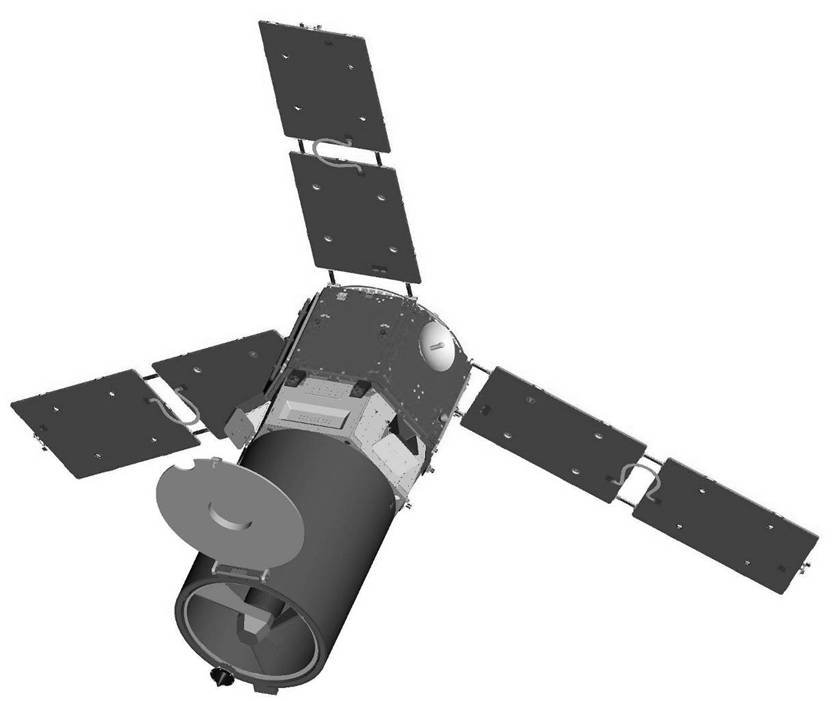
\includegraphics[width=\textwidth, height=0.3\textheight, keepaspectratio]{figures/ORS-1_graphic.jpg}

            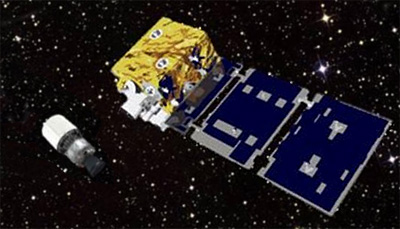
\includegraphics[width=\textwidth, height=0.3\textheight, keepaspectratio]{figures/angels__2.jpg}
        \end{column}
    \end{columns}
\end{frame}

\begin{frame}{Course Outcomes}
    \begin{itemize}
        \item By the end of the course
            \begin{itemize}
                \item Write programs to solve basic engineering problems in astronautics
                \item Develop structured code in a high-level programming language
                \item Document programs so they are easier to maintain and modify
                \item Debug and test in a systematic fashion to ensure code is correct
                \item Create library of code to perform common astrodynamic functions
            \end{itemize}
    \end{itemize}
\end{frame}

\begin{frame}{Getting Help}
    \begin{itemize}
        \item For most (if not all) students, this course will be extremely challenging:
            \begin{itemize}
                \item New content - astrodynamics and Python
                \item Structured programming - systematic, documentation, unit testing
                \item Technical writing 
            \end{itemize}
        \item Answers to your problems will rarely if ever be given to you. 
            You'll need to discover and learn these skills through focused effort.
            You have several sources of help:
            \begin{itemize}
                \item Instructor
                \item Classmates - may ask each other for help.
                \item ALL WORK MUST BE YOUR OWN.
                    \begin{itemize}
                        \item Copying
                        \item ``Working together``
                        \item Plagiarizing
                    \end{itemize}
                \item Textbooks/Internet - reference not copying
            \end{itemize}
    \end{itemize}
\end{frame}

\end{document}

